\documentclass[11pt]{article}
\usepackage{graphicx}
\usepackage{float}

%opening
\title{}
\title{%
	Extended public key cryptography in OpenSSL\\
	\large HW6-7 - CNS Sapienza}
\author{Giulia Muscarà 1743261}
\date{December 19, 2019}

\begin{document}

\maketitle
\section{Objectives}
The purpose of this report is to present and analyze some OpenSSL tools for public key cryptography. In particular, the focus is on RSA and DSA asymmetric encryption protocols. Public and private keys were generated, along with X.509 digital certificates and digital signatures. Then a virtual network was created using Netkit environment to simulate the exchange of messages between a Certificate Authority and a host, to request and receive certificates' signatures and revocations. To carry out the analysis, the commands were executed on a scriptable Bash shell running on a Lubuntu Netkit virtual box, as it provides a fast and lightweight operating system with a clean and easy-to-use user interface and it allows to emulate a network. \\

\section{Private key generation}
To generate a private key, OpenSSL offers, among others, the command \textit{genpkey}. By command line, it requires the specification of the desired algorithm to be used and the name of the output file \textit{.pem} where the key will be stored. In this case, two private keys were generated, one by using DSA and the other by using RSA, using the default cipher and operating mode for both of them. While for RSA private key the above said options are sufficient, DSA protocol also requires the specification of the \textit{-paramfile}, with a \textit{.pem} file containing the necessary parameters to compute the key. To randomly generate the parameters, beforehand the command \textit{genpkey} was used with the option \textit{-genparam} to produce the needed file \textit{dsaparams.pem} with 1024-bit long parameters, so that the dsa key could be computed starting from them.
After being created, the two private keys were stored in the respective files \textit{private\_rsa.pem} and \textit{private\_dsa.pem}.

\begin{figure}[H]
	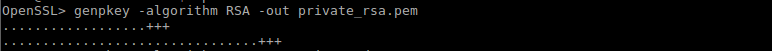
\includegraphics[width=1\textwidth]{img1-hw6-1743261.png}
	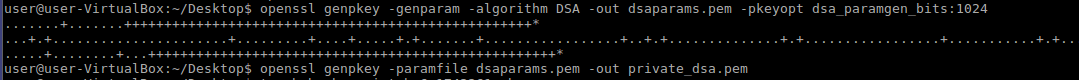
\includegraphics[width=1\textwidth]{img2-hw6-1743261.png}
	\caption{RSA and DSA private keys generation}
\end{figure}

\section{Public key extraction}
The previously generated private keys include the respective public ones, that were extracted from the files containing the private keys. \\
As far as the rsa private key was concerned, to extract the public RSA one, \textit{rsa} OpenSSL command was used. In particular, through \textit{-in} and \textit{-pubout -out} options, from the file containing the private key, another \textit{.pem} file was created, storing in it the associated RSA public key.
The same procedure was carried out for the extraction of DSA public key. This time, \textit{dsa} command was adopted with the same options specified for RSA. The two public keys were stored in the respective files \textit{public\_rsa.pem} and \textit{public\_dsa.pem}.

\begin{figure}[H]
	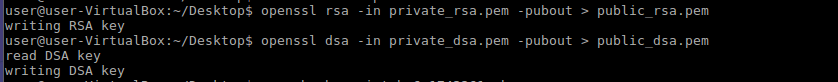
\includegraphics[width=1\textwidth]{img3-hw6-1743261.png}
	\caption{DSA and RSA public keys extraction}
\end{figure}

\section{X.509 certificate generation}
Then, X.509 digital certificates were created and verified by self-signing it. X.509 standard defines the format of public key certificates. Certificates contain a public key and the related identity, and it is either signed by a certificate authority or self-signed. 
In order to create an X.509 certificate, the \textit{req} OpenSSL command was used. The \textit{-new} option specified the request of a new Certificate Signing Request, the \textit{-key} option allows to specify a file containing an existing key and \textit{-out} is used to store in the \textit{rsa\_certificate\_req.csr} file the generated CSR. It was needed to insert a series of details about who is requesting the certificate, that in this case were left on default values, and a password challenge for the key by command line.

\begin{figure}[H]
	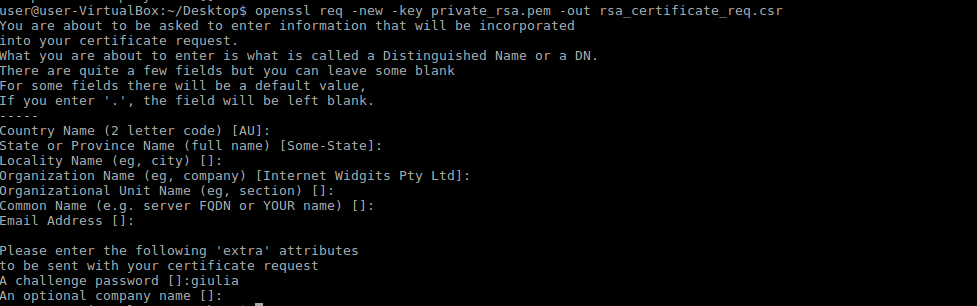
\includegraphics[width=1\textwidth]{img4-hw6-1743261.png}
	\caption{RSA certificate request}
\end{figure}

After creating a CSR, in order to self-sign the certificate, the private keys were used to prove the identity of the certificate owner. Through the command \textit{x509}, the CSR was signed with the private key and the number of days of validity were specified. After the verification, the \textit{rsa\_certificate.pem} file was created, which is the actual certificate. The content of the certificate was displayed as follows.\\

\begin{figure}[H]
	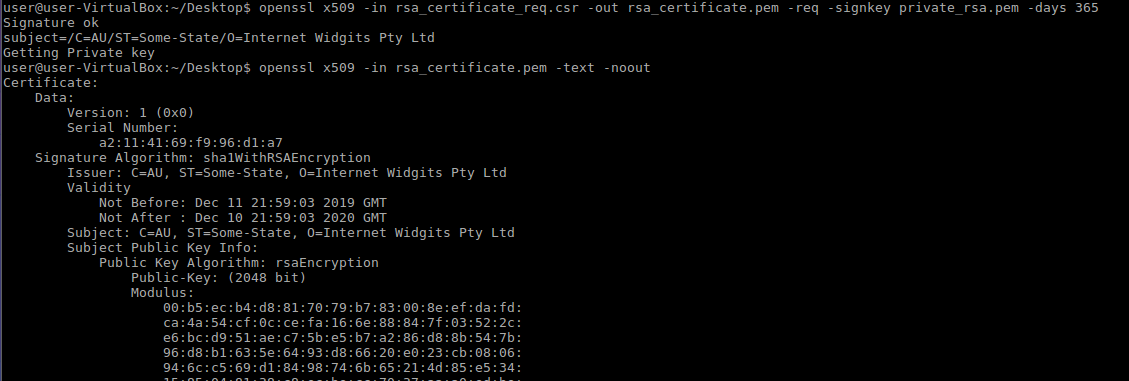
\includegraphics[width=1\textwidth]{img5-hw6-1743261.png}
	\caption{RSA certificate signing}
\end{figure}

The exact same procedure can be applied to create a certificate signed with the DSA private key.\\
Finally, in order to verify the created certificates, the \textit{verify} command was used, as shown in Fig. 5.

\begin{figure}[H]
	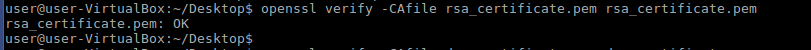
\includegraphics[width=1\textwidth]{img6-hw6-1743261.png}
	\caption{RSA certificate verification}
\end{figure}
\clearpage
The exact same procedure can be applied to verify a certificate signed with the DSA private key.\\

\section{Digital signatures}
Digital signatures securely associate a signer to its identity and a document. DSs come in the standard PKI format, to provide the highest levels of security and universal acceptance. While during a digital signature transaction the private key is not shared but it is used only by the signer to digitally sign documents, the public one is openly available and used by who needs to validate the authenticity of the digital signature. 
To digitally sign a sample empty document \textit{to\_sign.txt} in OpenSSl and to verify the signature, we need a pair \textit{(privatekey, publickey)}, which was already generated. 
By using the OpenSSL command \textit{dgst} with the option \textit{-sign}, the file \textit{sign.sha256} is created in the /tmp/ folder, containing the binary format of the digital signature, which was then encoded into the \textit{rsa\_digital\_signature.pem} file. On the other hand, to verify the signature, the public key was used. The verification consists in the inverse process: the \textit{rsa\_digital\_signature.pem} file was decoded into the \textit{sign.sha256} file and the latter was decrypted by using the public key. \textit{Verification OK} was printed, as the process ended correctly.

\begin{figure}[H]
	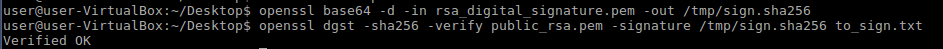
\includegraphics[width=1\textwidth]{img7-hw6-1743261.png}
	\caption{RSA signature verification}
\end{figure}
The exact same procedure can be applied to verify a digital signature created with a DSA private key.\\

\section{Certificate formats convertion}
There are different file extensions for X.509 certificates. Among the most used there are the \textit{.pem} format, that stands for Privacy-enhanced Electronic Mail and Base64 encoded, \textit{.cer, .crt, .der} formats, that indicate binary DER form, \textit{.p7b, .p7c}, for PKCS7 SignedData structure without data, just certificates or CRLs, and \textit{.p12}, which may contain certificates and private keys.\\
The certificates were previously created using PEM, in Base64 format, starting with "BEGIN CERTIFICATE" and "END CERTIFICATE". OpenSSL allows to convert certificates in other formats, like DER, which has a binary form. 
In particular, by using the \textit{x509} command PEM format files can be transformed into DER files and viceversa, by specifying the format of the file to convert with the option \textit{-inform} and the format of the desired output with the option \textit{-outform}.

\section{Network simulation}
To make a practical example of a host making requests and getting responses from an external CA, a virtual network was built up thanks to the Netkit environment. Netkit allows to set up and to perform networking experiments by creating several virtual network devices that can be interconnected. \\ The sample network is composed by two VMs, called v1 and v2, the former acting as a CA and the latter as a simple host, and by a router r that interconnects v1 and v2.
To make sure that each VM can communicate with the others and exchange files and requests the ICMP protocol was exploited, pinging the IP addresses of the terminals, that were chosen statically and randomly. The topology is characterized by the fact that the CA and the host are situated in two different LANs. The first subnet has address 192.168.0.0/24 and it is formed by v1 and the interface eth0 of the router, while the second LAN has address 10.0.0.0/24 and is made of v2 and the interface eth1 of r. The topology is shown in Fig. 7.\\
\begin{figure}[H]
	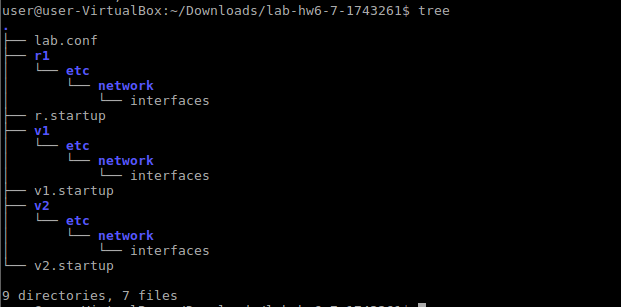
\includegraphics[width=1\textwidth]{img8-hw7-1743261.png}
	\caption{Network topology}
\end{figure}
\clearpage
After verifying that v1 was reachable from v2 through pings, because the \textit{openssl.cnf} file at \textit{v1/etc/ssl/openssl.cnf} specifies where the certificates, keys, crl, databases should be stored to be correctly managed when using OpenSSL, the necessary folders were created as well.\\
\begin{figure}[H]
	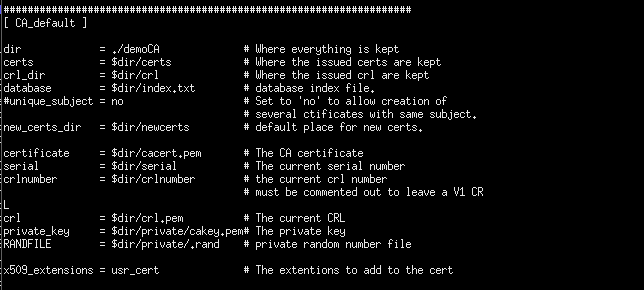
\includegraphics[width=1\textwidth]{img9-hw7-1743261.png}
	\caption{Folders structure}
\end{figure}
To make v1 a CA, its private key was generated using the \textit{genrsa} function and it was moved to the \textit{/CADemo/private/} folder. 
\begin{figure}[H]
	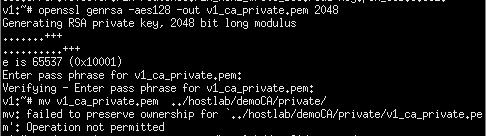
\includegraphics[width=1\textwidth]{img10-hw7-1743261.png}
	\caption{CA private key generation}
\end{figure}
Then a self-signed certificate for the CA was created, to distribute it to all the hosts of the network that need to trust v1, propagating it to v2 through the network.\\
\begin{figure}[H]
	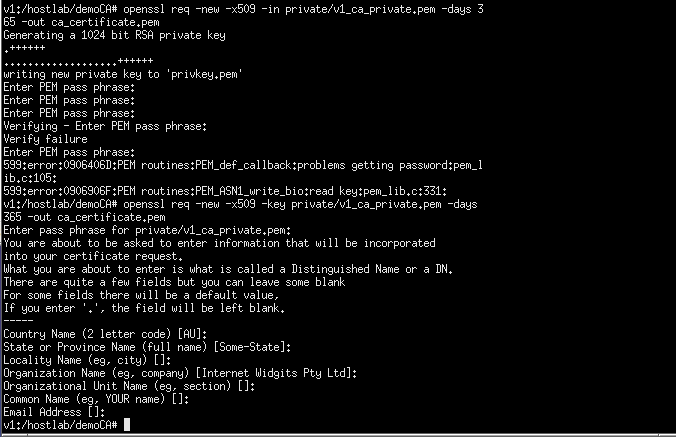
\includegraphics[width=1\textwidth]{img11-hw7-1743261.png}
	\caption{CA's self-signed certificate}
\end{figure}
As far as v2 is concerned, after receiving the CA's certificate, its private key was generated as well as a CSR for the CA, using the ip address of v2 as domain name. During the creation of the CSR, the fields of the common name and the email were specified as v2 and v2@vm.com respectively. After its creation, the \textit{.csr} file was sent to the CA through the network.\\
\begin{figure}[H]
	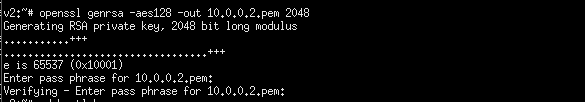
\includegraphics[width=1\textwidth]{img12-hw7-1743261.png}
	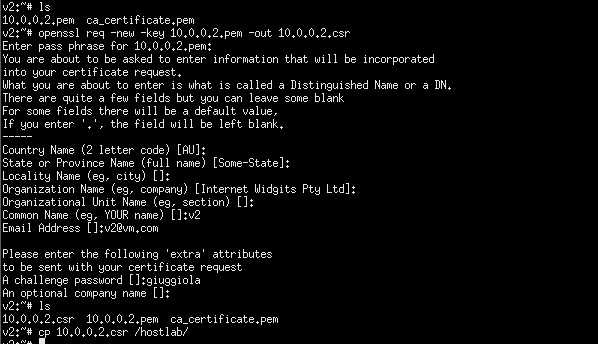
\includegraphics[width=1\textwidth]{img13-hw7-1743261.png}
	\caption{Host private key and csr creation}
\end{figure}

\section{Signature}
Now the CA can sign v2's certificate. By pressing ”y” the certificate was signed and the database updated with an entry representing this certificate.  The CA saved automatically a copy of the certificate, stored in the folder \textit{newcerts}, where each certificate is named with its timestamp, so in this case we have 01.pem. \\
\begin{figure}[H]
	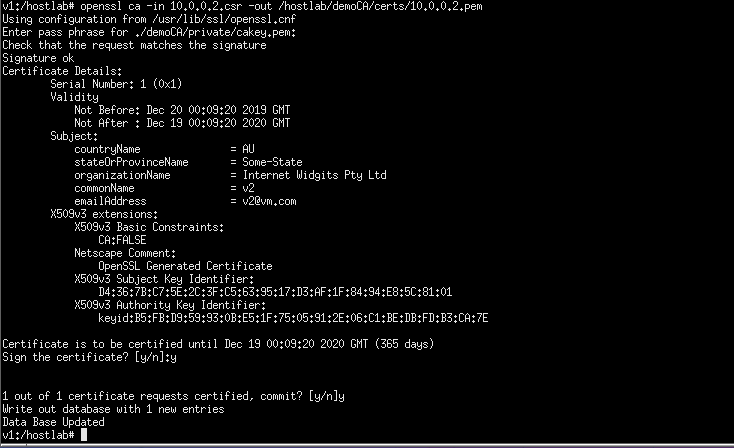
\includegraphics[width=1\textwidth]{img14-hw7-1743261.png}
	\caption{Certificate signing}
\end{figure}
After sending a copy of the signed certicate to V2, it can finally verify the certificate by using the public key of v1 contained in the cacert.pem certificate.\\
\begin{figure}[H]
	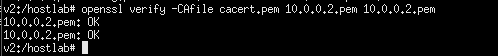
\includegraphics[width=1\textwidth]{img15-hw7-1743261.png}
	\caption{Certificate verification}
\end{figure}

\section{Revocation}
To revocate v2's certificate the following command were executed.
\begin{figure}[H]
	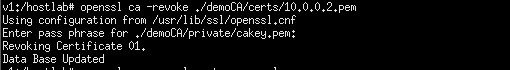
\includegraphics[width=1\textwidth]{img16-hw7-1743261.png}
	\caption{Certificate revocation}
\end{figure}
The file \textit{index.txt} was updated, indicating that the certificate in question has been revoked. Finally, a new CRL was created.
\begin{figure}[H]
	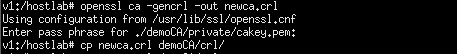
\includegraphics[width=1\textwidth]{img17-hw7-1743261.png}
	\caption{Certificate creation}
\end{figure}

\end{document}